\section{Other transducers}

\textit{Not really important for the exam. Just to understand the concepts, no need to know all the working sensors.}

\subsection{Motion and occupancy}

\begin{itemize}
    \item Air pressure sensor (doors, windows opening)
    \item Capacitance of the human body
    \item Acoustic, sounds level
    \item Photoelectric/photodiode/phototransistor when passing in front of a light source
    \item Pressure switch
    \item Stress/strain gauge
    \item Mechanical or magnetic switches sensors
    \item Vibration sensors
    \item Glass breakage sensor
    \item IR sensor (thermal vision)
    \item Microwave detector
    \item Ultrasonic sensors
    \item Video and image treatment
    \item Triboelectric sensors
\end{itemize}

\subsubsection{Microwave/RADAR sensors}

The microwave detectors offer an attractive alternative to other detectors when it is
required to cover large areas and to operate over an extended temperature range under
the influence of strong interferences, such as wind, acoustic noise, fog, dust, moisture,
and so forth. These detectors (sensors) belong to the active sensors as they provide an
excitation signal. That is, they emit pulses of the electromagnetic energy. The
operating principle of a microwave detector is based on radiation of electromagnetic
radiofrequency (RF) waves toward a protected area. The reflected waves are received,
amplified, and analyzed. A \textbf{time delay} between the sent (pilot) signal and received
reflected signal is used to measure \textbf{distance} to the object, while the \textbf{frequency shift} is
used to measure \textbf{speed of motion} of the object.

\begin{minipage}{0.45 \linewidth}
\begin{figure}[H]
    \centering
    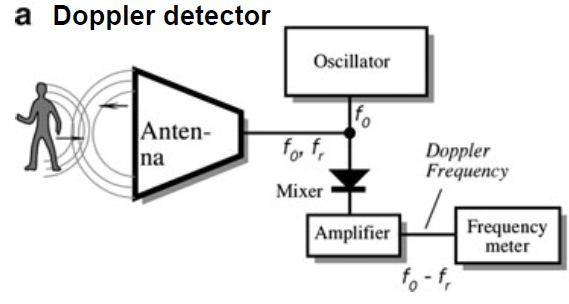
\includegraphics[width = 0.8 \textwidth]{L7/img/doppler-detector.PNG}
\end{figure}
\end{minipage}\hfill
\begin{minipage}{0.45 \linewidth}
Recall that for the Doppler effect we have $$\Delta f = f_0 - f_r = f_0 \frac{1}{1+c_0/v}$$
And, since $c_0/v\gg 1$, we have $$ \Delta f = \frac{v}{\lambda_0} $$ 
Therefore, the signal frequency at the output of the mixer is linearly proportional
to the velocity of a moving target. 

The \textbf{Gunn oscillator} is a diode mounted in a small precision cavity,
which, upon application of power, oscillates at microwave frequencies.
\end{minipage}

\subsubsection{Triboelectric detector}

\begin{minipage}{0.5 \linewidth}
\begin{figure}[H]
    \centering
    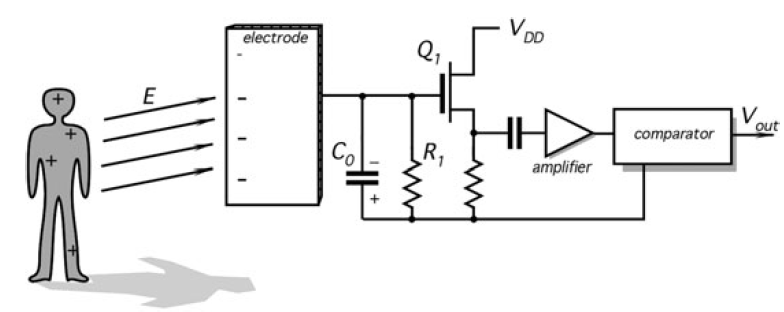
\includegraphics[width = 0.6 \textwidth]{L7/img/triboelectric.PNG}
\end{figure}
\end{minipage}\hfill
\begin{minipage}{0.5 \linewidth}
Any object can accumulate, on its surface, static electricity.
A static electric field is disturbed if a charge carrier (a human or an animal) changes its position and moves away
or if a new charge-carrying object enters into the vicinity of the electrode.

This kind of sensor is quite sensitive to the 50 Hz, EM fields, lightning, \dots
\end{minipage}


\subsection{Flow sensors}

\subsection{Acoustic and sound}

\subsection{Radiation sensors}

\subsection{Bio/Chemical sensors}

\subsection{Materials and technologies}
